\section{Supplemental Material}

\subsection{List of Features}

We provide a list of all of the input features used in the model, grouped by source. Note that all features are spatially aggregated to the county level, using a weighted average (where each grid cell is weighted by the fraction of the cell that lies inside the county, multiplied by the percentage of the grid cell that is cropland/pasture/grassland). An example of this aggregation process is depicted in Figure \ref{aggregating_to_county}. Temporally, all time-dependent features are also aggregated to weekly frequency.

\begin{figure}[h]
\centering
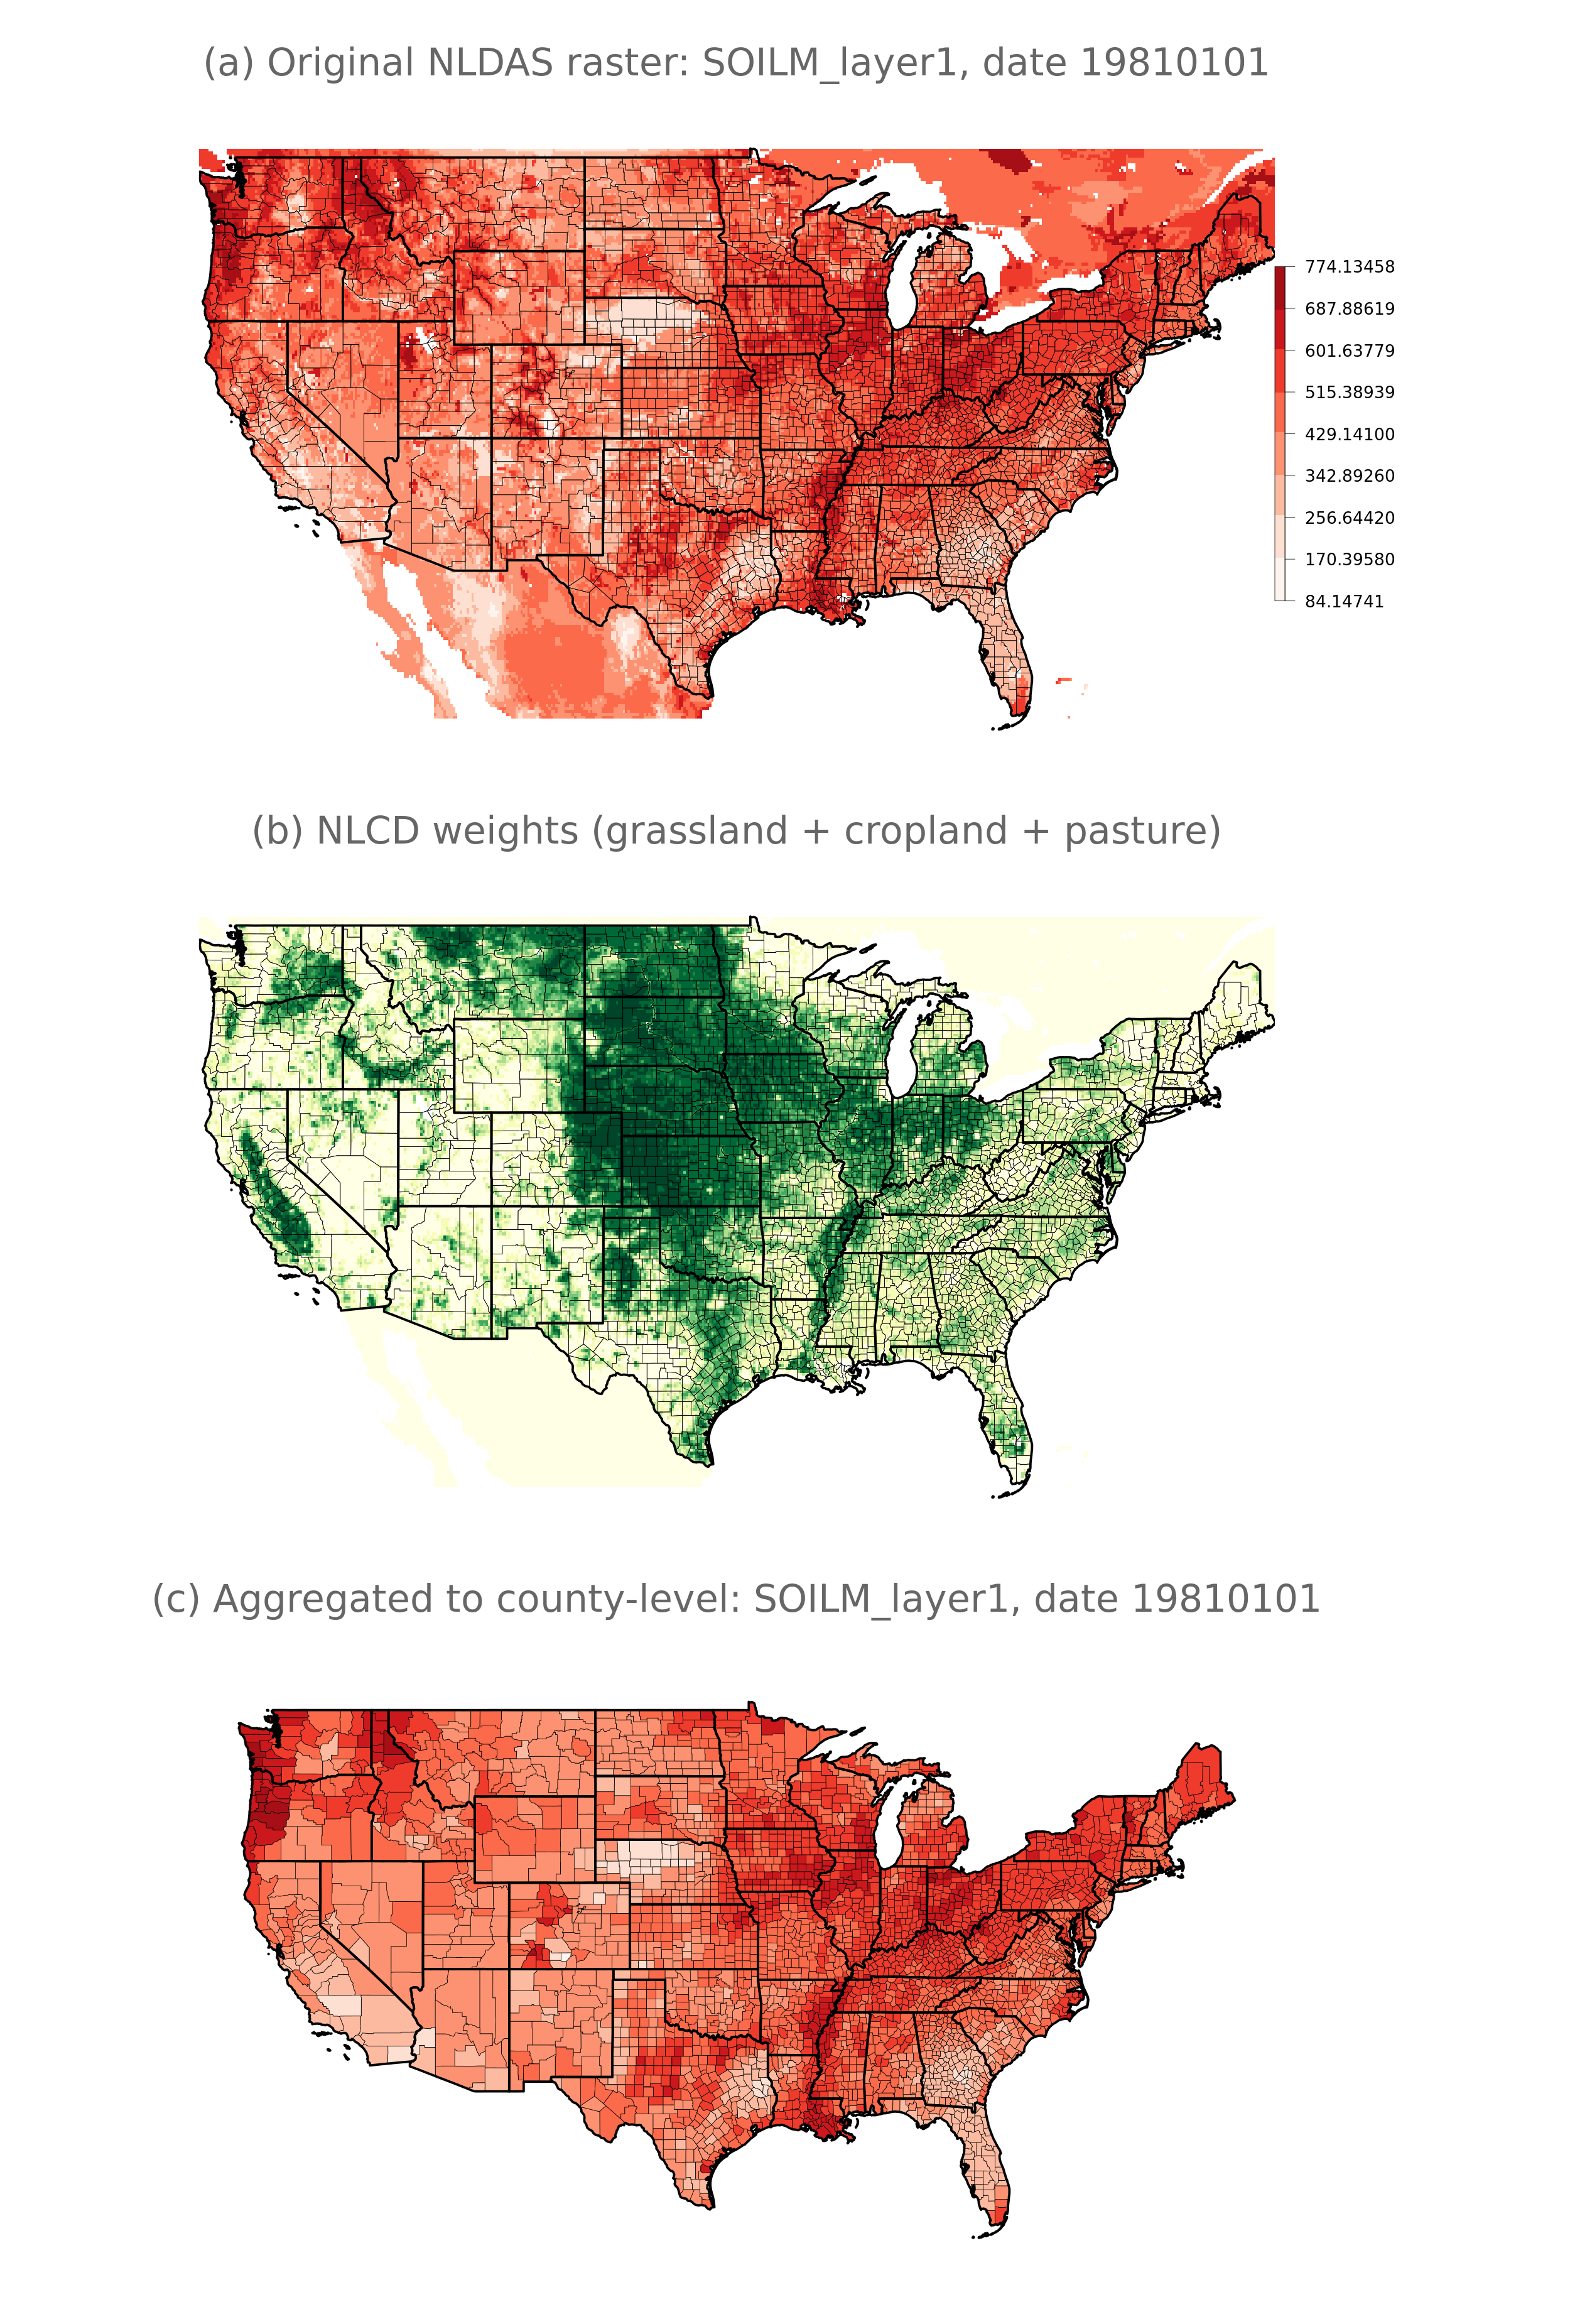
\includegraphics[width=0.9\columnwidth]{figs/nldas_SOILM_layer1_19810101_raster_and_weights.png}
\caption{Example of aggregating features to county level. \\
\textbf{(a)} raw raster of soil moisture from NLDAS. \\
\textbf{(b)} Percentage cropland/grassland/pasture (used to compute grid cell weights).\\
\textbf{(c)} the county-level values we generated.}
\label{aggregating_to_county}
\end{figure}


\textbf{Weather features} ($\mathbf{x}_{c,t}^w$) come from the PRISM dataset \cite{daly2013prism}, with an original spatial resolution of 4 km and a temporal resolution of daily:

\begin{enumerate}
    \item Precipitation
    \item Mean dewpoint temperature
    \item Daily max temperature
    \item Daily mean temperature
    \item Daily minimum temperature
    \item Max vapor pressure deficit
    \item Min vapor pressure deficit
\end{enumerate}

\textbf{Land surface features} ($\mathbf{x}_{c,t}^l$) come from the NLDAS land surface model \cite{xia2012continental}, with an original spatial resolution of 0.125 degrees (14 km) and a temporal resolution of hourly:

\begin{enumerate}
    \item Precipitation hourly total (kg/$m^2$)
    \item Moisture availability (\%), 0-200 cm
    \item Moisture availability (\%), 0-100 cm
    \item Soil moisture content (kg/$m^2$), 0-200cm
    \item Soil moisture content (kg/$m^2$), 0-100cm
    \item Soil moisture content (kg/$m^2$), 0-10cm
    \item Soil moisture content (kg/$m^2$), 10-40cm
    \item Soil moisture content (kg/$m^2$), 40-100cm
    \item Soil moisture content (kg/$m^2$), 100-200cm
    \item 2-m above ground specific humidity (kg/kg)
    \item 2-m above ground temperature (K)
    \item Soil temperature (K), 0-10 cm
    \item Soil temperature (K), 10-40 cm
    \item Soil temperature (K), 40-100 cm
    \item Soil temperature (K), 100-200 cm
    \item Wind speed (m/s), hourly max
\end{enumerate}

(Note that the cm ranges represent depths in the soil.)\\

 \textbf{Soil quality features} ($\mathbf{x}_{c}^s$) come from the Gridded Soil Survey Geographic Database (gSSURGO) \cite{soil2019gridded}. The dataset has a 30-m spatial resolution for the continental U.S. These variables do not change over time. However, they vary with depths, which are measured at 6 soil depth layers (0-5cm, 5-15cm, 15-30cm, 30-60cm, 60-100cm, 100-200cm). Because soil quality at a given point can vary substantially within a county, accounting for the location of agricultural activity can be critical when constructing appropriate county-level soil variables. Thus, the ``weighted-average'' technique is especially important here. We aggregate the fine-scale soil data to the county level based on the percentage of each NLCD Land Cover grid cell that was covered by agricultural land (grassland, pasture, cropland) in 2011.
 
\begin{enumerate}
    \item Available water capacity of the dominant soil component
    \item Bulk density
    \item Electrical conductivity of the dominant soil component
    \item Organic matter
    \item Average \% silt
    \item Average \% clay
    \item Average \% sand
    \item \% area covered by Clay soil type
    \item \% area covered by Silty Clay soil type
    \item \% area covered by Sandy Clay soil type
    \item \% area covered by Clay Loam soil type
    \item \% area covered by Silty Clay Loam soil type
    \item \% area covered by Sandy Clay Loam soil type
    \item \% area covered by Loam soil type
    \item \% area covered by Silt Loam soil type
    \item \% area covered by Sandy Loam soil type
    \item \% area covered by Silt Loam soil type
    \item \% area covered by Loamy Sand soil type
    \item \% area covered by Sand soil type
    \item pH, which is influenced by chemical reactions between water and the dominant soil component
\end{enumerate}
Note that features 8-19 were not present in the original gSSURGO dataset. Rather, for each pixel, we used the raw silt, clay, and sand percentages to compute the ``soil texture type'' of that pixel, based on the National Resources Conservation Service Soil Survey's classification scheme \cite{soiltexture}. This classification scheme is depicted in Figure \ref{soil_triangle}. After classifying each pixel's soil texture type, we compute the fraction of each county that is occupied by each soil texture type.

\begin{figure}[bt]
\centering
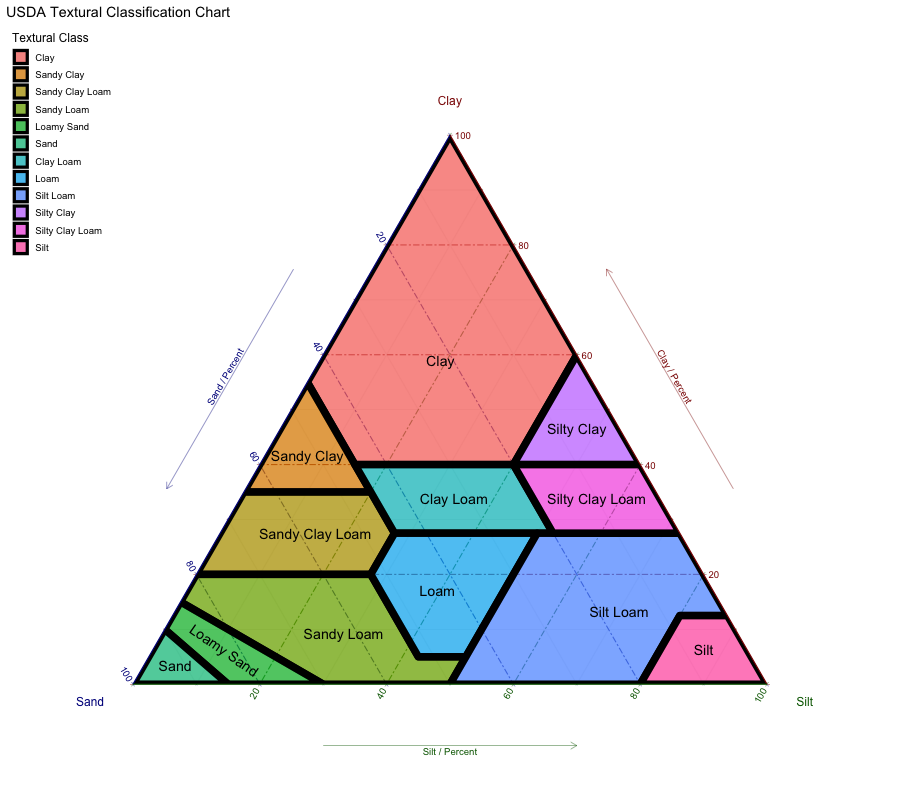
\includegraphics[width=0.95\columnwidth]{figs/soil_triangle.png}
\caption{NRCS Soil Texture classification \cite{soiltexture}. The three sides of the triangle represent percentage sand, clay, and silt, and the colored regions are the soil texture types.}
\label{soil_triangle}
\end{figure}

\textbf{Extra features} ($\mathbf{x}_{c}^e$) also come from the gSSURGO dataset \cite{soil2019gridded}, but are not depth-dependent. They are listed below:

\begin{enumerate}
    \item National commodity crop productivity index
    \item Depth to any soil restrictive layer
    \item NCCPI crop productivity index for small grains, weighted average
    \item NCCPI crop productivity index for corn
    \item NCCPI crop productivity index for cotton
    \item NCCPI crop productivity index for soybean
\end{enumerate}
% \begin{table}[]
% \centering
% % \fontsize{9}{10}\selectfont
% \begin{tabular}{|l|c|c|c|} \hline
% \textbf{Data source} & \textbf{Original temporal resolution} & \textbf{Original spatial resolution} & \textbf{Features} \\ \hline
% PRISM & & & \\
% \end{tabular}
% \caption{2019 soybean results}
% \label{2019_soybean}
% \end{table}




\subsection{Hyperparameter Details}

For all methods, we use the Adam optimizer \cite{kingma2014adam}. For the CNN-RNN, GNN, and GNN-RNN methods, we tried many hyperparameter configurations, most intensively on the 2018 corn dataset. We tried learning rates from \{1e-5, 2e-5, 5e-5, 1e-4, 2e-4, 5e-4, 1e-3\}, used a weight decay of 1e-5 or 1e-4, and a batch size of 32, 64, or 128. We tried using a mild cosine decay (with $\eta_{min} \in $ \{1e-5, 1e-6\}, $T_0 \in \{34, 100, 200\}$), or step decay (every 25 epochs, $\gamma \in \{0.5, 0.8\}$) for the learning rate scheduler. We trained the model for 100 to 200 epochs (until the validation loss clearly stopped improving). We chose the epoch and hyperparameter setting that produced the lowest RMSE on the validation year (the year before the test year).

For the GNN and GNN-RNN models, we used the implementation of GraphSAGE from the dgl library; we used a 2-layer GNN, with edge dropout of 0.1. We used stochastic mini-batch training to train the model, where each layer samples 10 neighbors to receive messages from. We tried different aggregation functions, such as ``mean'' and ``pooling.''



We ran the GNN-RNN model 3 times with random seeds \{0, 1, 2\} to evaluate the variance in the results. For the baseline models, we used seed 0. The final hyperparameter configurations are listed in the below tables.

% main.py --dataset corn_weekly --data_dir /mnt/beegfs/bulk/mirror/jyf6/datasets/crop_forecast/data/combined_dataset_weekly.npz -adj ../map/us_adj.pkl --crop_id_to_fid ../map/soybean_fid_dict.pkl --mode train --length 5 -bs 128 --max_epoch 100 --test_year 2019 --model cnn_rnn -lr 1e-4 --eta_min 1e-5 --check_freq 80 --T0 50 -sche step --crop_type corn --num_weather_vars 23 --num_management_vars 96 --num_soil_vars 20 --num_extra_vars 6 --soil_depths 6
\begin{table}[H]
\centering
% \fontsize{9}{10}\selectfont
\begin{tabular}{|l|l|} \hline
\textbf{Hyperparameter} & \textbf{Value} \\ \hline
Batch size & 128 \\ \hline
Learning rate & 1e-4\\ \hline
LR scheduling & Step (25 epochs, $\gamma$ = 0.5)  \\ \hline
Number of epochs & 100 \\ \hline
Weight decay & 1e-5 \\ \hline
\end{tabular}
\caption{CNN-RNN hyperparameters: corn}
\label{hyperparams_cnn-rnn_corn}
\end{table}

\begin{table}[H]
\centering
% \fontsize{9}{10}\selectfont
\begin{tabular}{|l|l|} \hline
\textbf{Hyperparameter} & \textbf{Value} \\ \hline
Batch size & 128 \\ \hline
Learning rate & 5e-4 \\ \hline
LR scheduling & Step (25 epochs, $\gamma$ = 0.5)  \\ \hline
Number of epochs & 100 \\ \hline
Weight decay & 1e-5 \\ \hline
\end{tabular}
\caption{CNN-RNN hyperparameters: soybeans}
\label{hyperparams_cnn-rnn_soybean}
\end{table}

% python main.py --dataset corn_weekly --data_dir /mnt/beegfs/bulk/mirror/jyf6/datasets/crop_forecast/data/combined_dataset_weekly.npz  \
%     -adj ../map/us_adj.pkl --crop_id_to_fid ../map/soybean_fid_dict.pkl \
%     --mode train --length 5 -bs $1 --max_epoch 70 --test_year 2018 -lr $2 \
%     --eta_min 1e-5 --check_freq 80 --T0 200 -sche $3 --dropout 0.1 --z_dim 64 \
%     --crop_type corn --num_weather_vars 23 --num_management_vars 96 --num_soil_vars 20 --num_extra_vars 6 --soil_depths 6 --no_management --aggregator_type $4 \
%     --note $5
%./run_train.sh 32 1e-4 cosine pool day_0
\begin{table}[H]
\centering
% \fontsize{9}{10}\selectfont
\begin{tabular}{|l|l|} \hline
\textbf{Hyperparameter} & \textbf{Value} \\ \hline
Batch size & 32 \\ \hline
Learning rate & 1e-4 \\ \hline
LR scheduling & Cosine ($T_0 = 200, \eta_{min} = 10^{-5}$)  \\ \hline
Number of epochs & 100 \\ \hline
Weight decay & 1e-5 \\ \hline
GNN edge dropout & 0.1 \\ \hline
GNN aggregator & pool \\ \hline
\end{tabular}
\caption{GNN hyperparameters: corn, 2018}
\label{hyperparams_gnn_corn_2018}
\end{table}

% % "python main.py --dataset corn_weekly --data_dir /mnt/beegfs/bulk/mirror/jyf6/datasets/crop_forecast/data/combined_dataset_weekly.npz  \
%     -adj ../map/us_adj.pkl --crop_id_to_fid ../map/soybean_fid_dict.pkl \
%     --mode train --length 5 -bs $1 --max_epoch 200 --test_year 2019 -lr $2 \
%     --eta_min 1e-5 --check_freq 80 --T0 100 -sche $3 --dropout 0. --z_dim 64 \
%     --crop_type corn --num_weather_vars 23 --num_management_vars 96 --num_soil_vars 20 --num_extra_vars 6 --soil_depths 6 --no_management \
%     --note $4
% # ./run_train.sh 64 5e-5 cosine day_0"
\begin{table}[H]
\centering
% \fontsize{9}{10}\selectfont
\begin{tabular}{|l|l|} \hline
\textbf{Hyperparameter} & \textbf{Value} \\ \hline
Batch size & 64 \\ \hline
Learning rate & 5e-5 \\ \hline
LR scheduling & Cosine ($T_0 = 100, \eta_{min} = 10^{-5}$)  \\ \hline
Number of epochs & 200 \\ \hline
Weight decay & 1e-5 \\ \hline
GNN edge dropout & 0 \\ \hline
GNN aggregator & mean \\ \hline
\end{tabular}
\caption{GNN hyperparameters: corn, 2019}
\label{hyperparams_gnn_corn_2019}
\end{table}


% model/soybeans_weekly/2018/gnn_bs-64_lr-0.0001_maxepoch-100_sche-step_T0-25_step-25_gamma-0.8_dropout-0.1_testyear-2018_aggregator-pool_encoder-cnn_trainweekstart-52_len-5_seed-1_no-management/model-58
% model/soybeans_weekly/2019/gnn_bs-64_lr-0.0001_maxepoch-100_sche-step_T0-25_step-25_gamma-0.8_dropout-0.1_testyear-2019_aggregator-pool_encoder-cnn_trainweekstart-52_len-5_seed-2_no-management/model-15
\begin{table}[H]
\centering
% \fontsize{9}{10}\selectfont
\begin{tabular}{|l|l|} \hline
\textbf{Hyperparameter} & \textbf{Value} \\ \hline
Batch size & 64 \\ \hline
Learning rate & 1e-4 \\ \hline
LR scheduling & Step (25 epochs, $\gamma = 0.8$)  \\ \hline
Number of epochs & 100 \\ \hline
Weight decay & 1e-5 \\ \hline
GNN edge dropout & 0.1 \\ \hline
GNN aggregator & pool \\ \hline
\end{tabular}
\caption{GNN hyperparameters: soybeans, 2018 and 2019}
\label{hyperparams_gnn_soybeans_2018}
\end{table}

% model/corn_weekly_no_Y_input_shuffle/2018/gnn-rnn_bs-32_lr-5e-05_maxepoch-100_sche-cosine_T0-100_etamin-1e-06_step-25_gamma-1.0_dropout-0.1_sleep-100_testyear-2018_aggregator-pool_encoder-cnn_trainweekstart-52_len-5_weightdecay-1e-05_seed-2_no-management/model-72
\begin{table}[H]
\centering
% \fontsize{9}{10}\selectfont
\begin{tabular}{|l|l|} \hline
\textbf{Hyperparameter} & \textbf{Value} \\ \hline
Batch size & 32 \\ \hline
Learning rate & 5e-5 \\ \hline
LR scheduling & Cosine ($T_0 = 100, \eta_{min} = 10^{-6}$)  \\ \hline
Number of epochs & 100 \\ \hline
Weight decay & 1e-5 \\ \hline
GNN edge dropout & 0.1 \\ \hline
GNN aggregator & pool \\ \hline
\end{tabular}
\caption{GNN-RNN hyperparameters: corn, 2018}
\label{hyperparams_gnn_corn_2018}
\end{table}

%model/corn_weekly_no_Y_input_shuffle/2019/gnn-rnn_bs-32_lr-5e-05_maxepoch-100_sche-cosine_T0-200_etamin-1e-06_step-25_gamma-1.0_dropout-0.1_sleep-100_testyear-2019_aggregator-pool_encoder-cnn_trainweekstart-52_len-5_weightdecay-1e-05_seed-2_no-management/model-88
\begin{table}[H]
\centering
% \fontsize{9}{10}\selectfont
\begin{tabular}{|l|l|} \hline
\textbf{Hyperparameter} & \textbf{Value} \\ \hline
Batch size & 32 \\ \hline
Learning rate & 5e-5 \\ \hline
LR scheduling & Cosine ($T_0 = 200, \eta_{min} = 10^{-6}$)  \\ \hline
Number of epochs & 100 \\ \hline
Weight decay & 1e-5 \\ \hline
GNN edge dropout & 0.1 \\ \hline
GNN aggregator & pool \\ \hline
\end{tabular}
\caption{GNN-RNN hyperparameters: corn, 2019}
\label{hyperparams_gnn_corn_2019}
\end{table}


%model/soybeans_weekly_no_Y_input_shuffle/2018/gnn-rnn_bs-32_lr-0.0001_maxepoch-100_sche-cosine_T0-100_etamin-1e-06_step-25_gamma-1.0_dropout-0.1_sleep-100_testyear-2018_aggregator-pool_encoder-cnn_trainweekstart-52_len-5_weightdecay-0.0001_seed-2_no-management/model-42
%
\begin{table}[H]
\centering
% \fontsize{9}{10}\selectfont
\begin{tabular}{|l|l|} \hline
\textbf{Hyperparameter} & \textbf{Value} \\ \hline
Batch size & 32 \\ \hline
Learning rate & 1e-4 \\ \hline
LR scheduling & Cosine ($T_0 = 100, \eta_{min} = 10^{-6}$)  \\ \hline
Number of epochs & 100 \\ \hline
Weight decay & 1e-4 \\ \hline
GNN edge dropout & 0.1 \\ \hline
GNN aggregator & pool \\ \hline
\end{tabular}
\caption{GNN-RNN hyperparameters: soybeans, 2018}
\label{hyperparams_gnn_soybeans, 2018}
\end{table}

%model/soybeans_weekly_no_Y_input_shuffle/2019/gnn-rnn_bs-32_lr-5e-05_maxepoch-100_sche-cosine_T0-100_etamin-1e-06_step-25_gamma-1.0_dropout-0.1_sleep-100_testyear-2019_aggregator-pool_encoder-cnn_trainweekstart-52_len-5_weightdecay-1e-05_seed-0_no-management/model-18
\begin{table}[H]
\centering
% \fontsize{9}{10}\selectfont
\begin{tabular}{|l|l|} \hline
\textbf{Hyperparameter} & \textbf{Value} \\ \hline
Batch size & 32 \\ \hline
Learning rate & 5e-5 \\ \hline
LR scheduling & Cosine ($T_0 = 100, \eta_{min} = 10^{-6}$)  \\ \hline
Number of epochs & 100 \\ \hline
Weight decay & 1e-5 \\ \hline
GNN edge dropout & 0.1 \\ \hline
GNN aggregator & pool \\ \hline
\end{tabular}
\caption{GNN-RNN hyperparameters: soybeans, 2019}
\label{hyperparams_gnn_soybeans, 2019}
\end{table}


\subsection{Evaluation Metrics}

We evaluate our model across all counties in the test year with data. We use three standard regression metrics: RMSE, $R^2$, and Pearson correlation coefficient (Corr). 

The RMSE is the square root of the mean squared error between the prediction and the true value:

$$RMSE = \sqrt{\frac{\sum_c (y_c - \widehat{y_c})^2}{N}}$$

where $y_c$ is the true yield for county $c$, $\widehat{y_c}$ is the model's predicted yield for county $c$, and $N$ is the total number for counties in the test set with yield data. In this paper, we further divide RMSE by the standard deviation of the current crop's yield (across all years), in order to make the results for different crops comparable.

$R^2$ is a measure of how much the variation in the data can be explained by the model predictions. Formally,

$$R^2 = 1 - \frac{\sum_c (y_c - \widehat{y_c})^2}{\sum_c (y_c - \bar{y})^2}$$

where $\bar{y}$ is the average yield across the entire test dataset. The top of the fraction is the sum of the squared residuals (difference between true yield and model prediction). The bottom is the total sum of squares (of the difference between the true yield and the average yield across the test dataset), which is proportional to the overall variance of the test data. 

The Pearson correlation coefficient (Corr) measures the strength of the linear correlation between the true and predicted values. The correlation between two variables $x$ and $y$ is given as

$$r_{xy} = \frac{\sum_{i=1}^n (x_i - \bar{x}) (y_i - \bar{y})}{\sqrt{\sum_{i=1}^n (x_i - \bar{x})^2} \sqrt{\sum_{i=1}^n (y_i - \bar{y})^2}}$$

Again $\bar{x}$ and $\bar{y}$ are the means of $x$ and $y$ respectively. We let $x$ be the model prediction and $y$ be the true yield.










\subsection{Data and Code Availability}

We are planning to submit an expanded version of this paper to a journal, such as in the field of agricultural economics. After the journal article is published, we plan to make the entire aggregated dataset and codebase publicly available. All of the raw data used comes from publicly available sources. For now, we have submitted a data appendix with a small subset of the aggregated county-level data (only the states of Illinois and Iowa), and a code appendix containing our implementation of the GNN-RNN model. 

\begin{figure}[t]
\centering
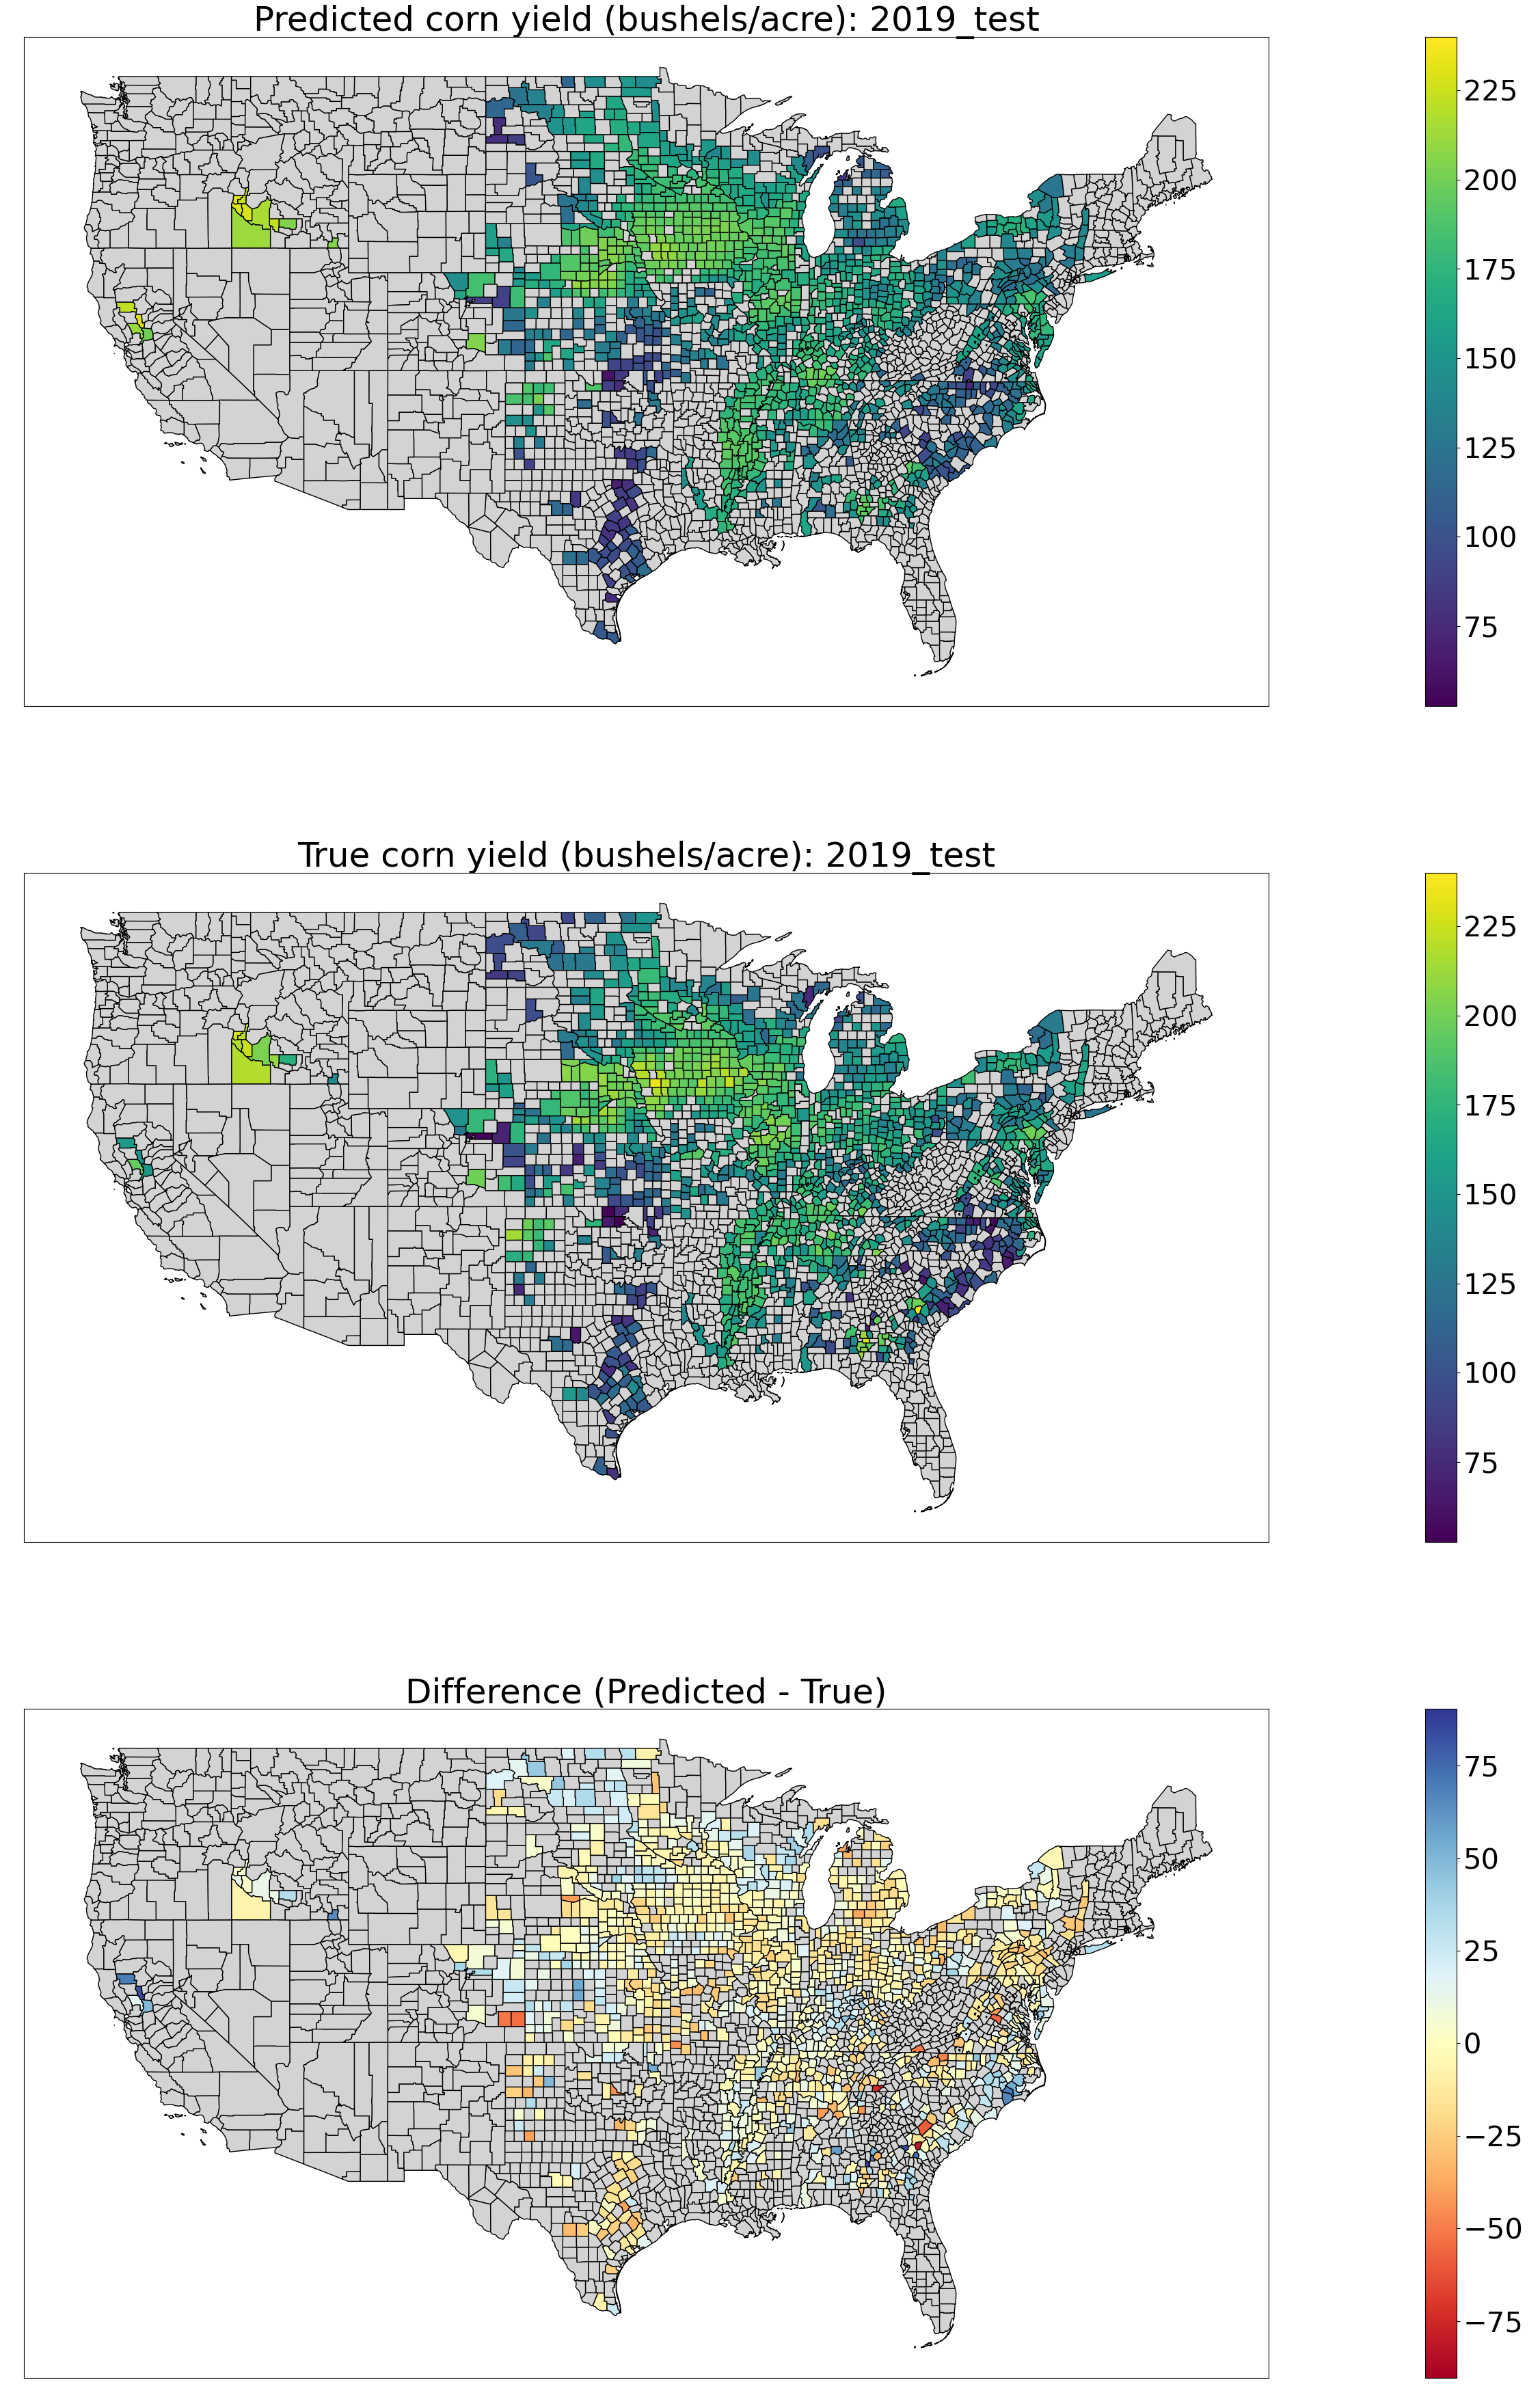
\includegraphics[width=0.95\columnwidth]{figs/true_vs_predicted_map_corn_2019_test.png}
\caption{2019 corn: Maps of predicted (top) and true (middle) yields, along with the difference (bottom).}
\label{fig:map_2019corn}
\vspace{-1em}
\end{figure}
\begin{figure}[H]
\centering
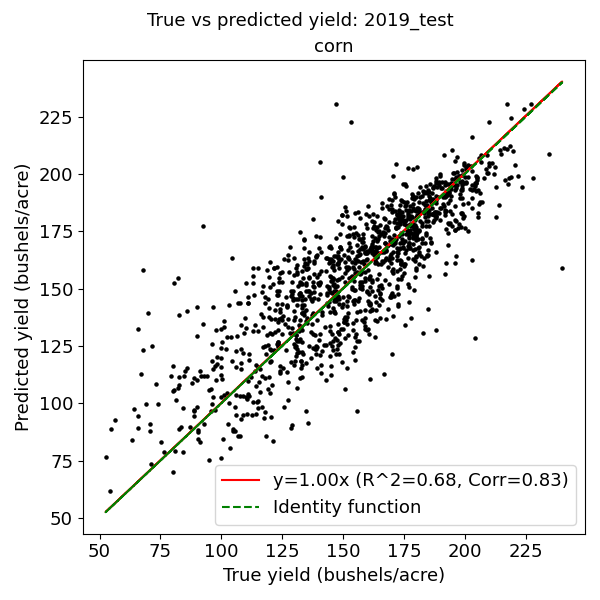
\includegraphics[width=0.8\columnwidth]{figs/true_vs_predicted_scatter_corn_2019_test.png}
\caption{2019 corn: Predicted vs. ground truth yields}
\label{fig:scatter_2019corn}
\end{figure}


\begin{figure}[H]
\centering
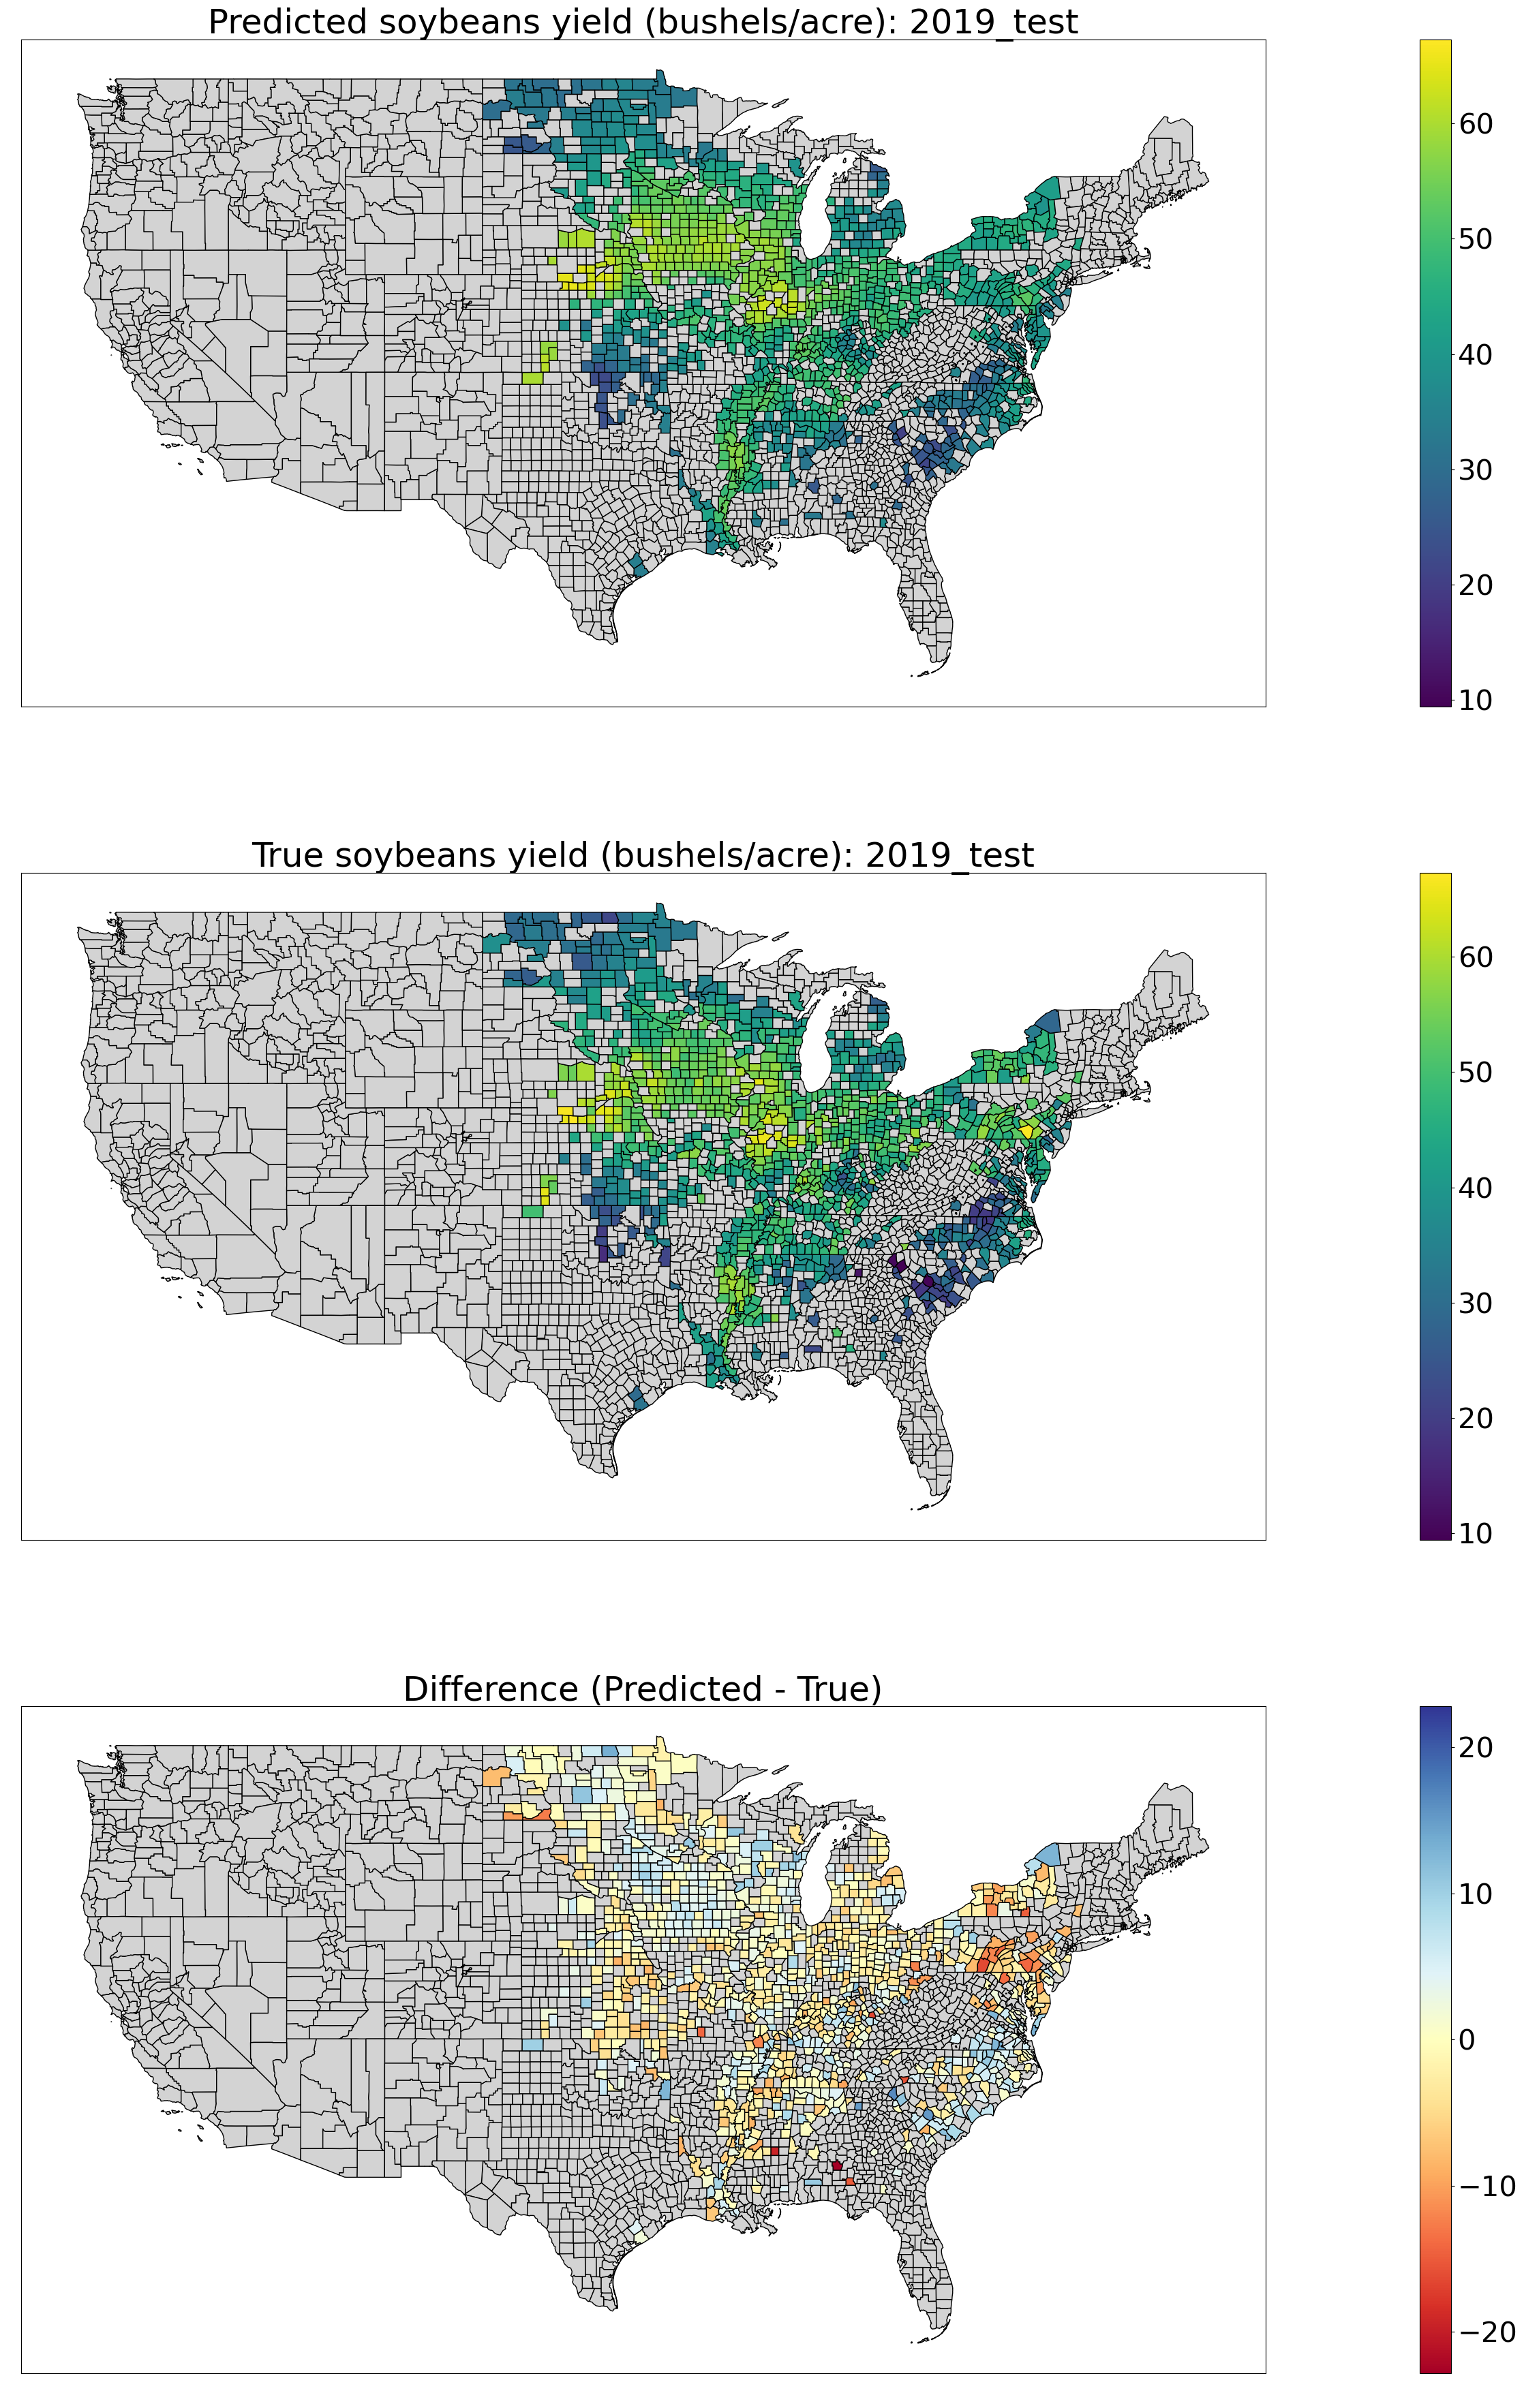
\includegraphics[width=0.95\columnwidth]{figs/true_vs_predicted_map_soybeans_2019_test.png}
\caption{2019 soybeans: Maps of predicted (top) and true (middle) yields, along with the difference (bottom).}
\label{fig:map_2019soy}
\end{figure}
\begin{figure}[H]
\centering
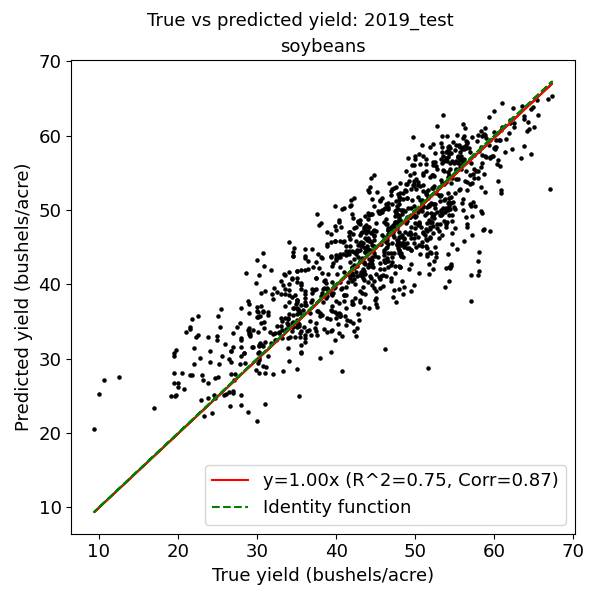
\includegraphics[width=0.8\columnwidth]{figs/true_vs_predicted_scatter_soybeans_2019_test.png}
\caption{2019 soybeans: Predicted vs. ground truth yields}
\label{fig:scatter_2019soy}
\end{figure}


\subsection{Computing Setup}

We ran our code on Python 3.7, using the following libraries: PyTorch 1.8, DGL 0.7.1, NumPy 1.18.5, SciPy 1.2.0. We trained on NVIDIA Tesla V100 GPU with 16GB memory, and used 12 CPU threads for GNN-RNN. The GNN-RNN model takes roughly 8 hours to train for 100 epochs on our full US dataset.



\subsection{Additional plots}

Here are maps and scatter plots showing example results for the GNN-RNN model on the other datasets.


\textbf{2019 corn:} Fig.~\ref{fig:map_2019corn} describes the difference between the ground-truth corn yields for counties in 2019, and our predictions. To demonstrate the similarity, we plot their difference in the bottom figure. As shown in the bottom sub-figure, almost all differences are all close to 0. Fig.~\ref{fig:scatter_2019corn} shows another plot of true-vs-predicted comparison. All the dots cling to the identity function, which means good prediction results.


\textbf{2019 soybeans:} Fig.~\ref{fig:map_2019soy} and Fig.~\ref{fig:scatter_2019soy} are similar true-vs-predicted plots for soybeans. The prediction results are also promising.




% \subsection{Early prediction results for soybean}

% Skip if not enough time